%UNDERSTANDING AREA \& UNIT SQUARES - WORKSHEET 3
\documentclass[12pt, letterpaper, fleqn]{article}

% ----------------------------------------------------------
% PACKAGES
% ----------------------------------------------------------
\usepackage{graphicx}
\usepackage{xcolor}
\usepackage[most]{tcolorbox}
\usepackage{amsmath, amssymb}
\usepackage{fancyhdr}
\usepackage[utf8]{inputenc}
\usepackage[T1]{fontenc}
\usepackage{enumitem}
\usepackage{geometry}
\usepackage{tikz}
\usepackage{needspace}
\usepackage{multicol}

\usetikzlibrary{arrows.meta, calc, shapes.geometric}

% ----------------------------------------------------------
% PAGE SETUP
% ----------------------------------------------------------
\usepackage{times}
\geometry{letterpaper, top=1.25in, bottom=1.25in, marginpar=0.5in}

% ----------------------------------------------------------
% HEADER / FOOTER
% ----------------------------------------------------------
\newcommand{\logowidth}{3cm}
\setlength{\headheight}{20pt}
\setlength{\footskip}{40pt}

\pagestyle{fancy}
\fancyhf{}
\fancyhead[C]{\small\bfseries Understanding Area \& Unit Squares}
\fancyfoot[L]{\raisebox{2pt}{
\includegraphics[width=\logowidth]{../kss.png}}}
\fancyfoot[C]{\thepage}
\fancyfoot[R]{3.22.3}

\renewcommand{\footrulewidth}{0.2pt}

% ----------------------------------------------------------
% THEME COLOR
% ----------------------------------------------------------
\definecolor{customteal}{HTML}{2fbdb9}

% ----------------------------------------------------------
% HELPER MACROS
% ----------------------------------------------------------
\newcommand{\blank}{\underline{\hspace{2.2cm}}}
\newcommand{\blanklong}{\underline{\hspace{6.5cm}}}
\newcommand{\blankshorter}{\underline{\hspace{1.5cm}}}

% ----------------------------------------------------------
% DOCUMENT
% ----------------------------------------------------------
\begin{document}

\textbf{Name:} \underline{\hspace{5cm}}
\hfill
\textbf{Date:} \underline{\hspace{3cm}}\\

\begin{tcolorbox}[colback=customteal!20]
    \large\textcolor{black}{\textbf{Quiz: Counting Area}}
\end{tcolorbox}

\vspace{5mm}
\begin{enumerate}[itemsep=3.5cm, leftmargin=0.6cm]
\item Find the area of the shaded shape by counting unit squares:
\\
\begin{tikzpicture}[scale=0.8]
\draw[step=1cm,gray,very thin] (0,0) grid (4,4);
\fill[customteal!30] (1,1) rectangle (3,3);
\fill[customteal!30] (3,2) rectangle (4,3);
\draw[step=1cm,gray,very thin] (0,0) grid (4,4);
\draw[thick] (0,0) rectangle (4,4);
\end{tikzpicture}
\\
Area: \blank square units

\item Draw a shape with an area of exactly **5 square units** on the grid below.
\\
\begin{tikzpicture}[scale=0.8]
\draw[step=1cm,gray,very thin] (0,0) grid (5,3);
\draw[thick] (0,0) rectangle (5,3);
\end{tikzpicture}
\end{enumerate}

\end{document}
